\documentclass[18pt]{beamer}
\usepackage[utf8]{inputenc}
\usepackage{xcolor}
\usepackage{hyperref}
\usepackage{templates/mytemplate}
\usepackage{templates/beamerthemekit}
\usepackage{graphicx}
\usepackage{microtype}
\usepackage{listings}
\usepackage{multicol}
\usepackage{siunitx}
\usepackage{physics}
\usepackage{appendixnumberbeamer}
\usepackage{booktabs}
\usepackage{longtable}
\usepackage{amssymb}
\usepackage{todonotes}
\usepackage{booktabs}
\usepackage[backend=biber, style=numeric]{biblatex}

\addbibresource{thesis.bib}
\lstset{ %
  backgroundcolor=\color{white},   % choose the background color; you must add \usepackage{color} or \usepackage{xcolor}; should come as last argument
  basicstyle=\tiny\ttfamily,
  xleftmargin=-10pt,
  breaklines=false,                 % sets automatic line breaking
  captionpos=b,                    % sets the caption-position to bottom
  % frame=single,	                   % adds a frame around the code
  keepspaces=true,                 % keeps spaces in text, useful for keeping indentation of code (possibly needs columns=flexible)
  language=C++,                 % the language of the code
  % morekeywords={*,...},            % if you want to add more keywords to the set
  tabsize=2,	                   % sets default tabsize to 2 spaces
  keywordstyle=\bfseries\color{kit-green70},
  commentstyle=\itshape\color{kit-blue70},
  identifierstyle=\color{black},
  stringstyle=\color{kit-orange100},  
}

\hypersetup{colorlinks=false, hidelinks=true, urlcolor=kit-blue100, %linkcolor=Firebrick4
}

\title{Einsichten in die Spurfindung an Belle II mit kosmischer Strahlung} 
\subtitle{Wissenschaftliches Schreiben und Präsentieren für Physiker und Metereologen}
\author{\underline{Michael Eliachevitch}}
\date{24. Januar 2018}
\titleimage{transparent}
\institute{}

\setbeamertemplate{bibliography item}{}
\begin{document}
\selectlanguage{ngerman}

\begin{frame}
  \titlepage
\end{frame}

\begin{frame}
  \frametitle{Was ist Belle II und wozu braucht man Spurfindung?}
  \begin{itemize}
    \item im Bau befindlicher Teilchendektor an dem SuperKEKB-Beschleuniger
    \item experimentelles Ziel: Beobachtung der Zerfälle B-Mesonen mit hoher Präzision
    \item physikalisches Ziel: Suche nach \emph{Physik jenseits des Standardmodells}
    \item Abweichungen der Zerfallsparameter von theoretischen Vorhersagen\\$\rightarrow$ \emph{neue Physik}?
    \item \emph{Spurfindung}: Rekonstruktion der Teilchenbahnen der aus Rohdaten des Detektors
    \end{itemize}
  \end{frame}

  

\begin{frame}
  \frametitle{Besonderheiten der Spurfindung an Belle II}
  \begin{itemize}
  \item SuperKEKB: Elektron-Positrion-Collider als \emph{B-Fabrik}\cite{Bevan:2014iga}:
    \begin{itemize}
    \item \emph{saubere} Ereignisse: wenig Untergrund, $\sim$7-11 Spuren 
    \item Kenntniss des Anfangszustandes: zwei B-Mesonen mit bekanntem Impuls
    \end{itemize}
  \end{itemize}
    \begin{itemize}
    \item Herausforderungen:
      \begin{itemize}
      \item Ziel: \emph{alle} Spuren in einem Ereignis finden $\rightarrow$ hohe \textbf{Effizienz}
      \item Kollisionsereignis etwa alle 4\,ns  \cite{Abe:2010gxa}
 $\rightarrow$ hohe \textbf{Performanz} der Algorithmen
      \end{itemize}
    \item Spurfindungs-Detektoren an Belle II:
      \begin{itemize}
      \item Vertexdetektor: noch nicht fertiggestellt
      \item \textbf{Driftkammer}: bereits funktionsfähig
      \end{itemize}
  \end{itemize}
  
\end{frame}

\begin{frame}
  \frametitle{Validierung der Spurfindung}
  \begin{itemize}
    \item Effizienz der Spurfindung: Anteil der Spuren, die gefunden werden
    \item bisherige Validierung: Monte Carlo-Simulationen
    \item Sommer 2017: Datennahme mit kosmischen Strahlen, größtenteils Myonen
      $\rightarrow$ Myonen: langlebige, schwach ionisierende Teilchen, die Materie durchdringen\cite{PDG}
    \end{itemize}
    \begin{block}{Idee}
      Ist es möglich, die  Spurfindung an Belle II mit kosmischen Myon zu validieren?
    \end{block}  
\end{frame}

\begin{frame}
  \frametitle{Prinzip: Datenbasierte Schätzung der Spurfindungs-Effizienz}
  \begin{itemize}    
  \item selektiere Myonen, die durch das leere Detektorzentrum gehen
  \item erfolgreiche Rekonstruktion: \textcolor{kit-blue100}{finde zwei Spuren}, obere Hälfte und untere Hälfte
  \item fehlgeschlagene Rekonstruktion: \textcolor{kit-red100}{finde nur eine Spur}
  \end{itemize}
  \begin{block}{}
    \begin{equation*}
      \label{eq:cosmic_eff}
      \text{Spurfindungs-Effizienz} = \frac{\textcolor{kit-blue100}{N_\mathrm{2\ Spuren\ gefunden}}}{N_\mathrm{2\ Spuren\ erwartet}}
      = 1 - \frac{\textcolor{kit-red100}{N_\mathrm{1\ Spur\ gefunden}}}{N_\mathrm{2\ Spuren\ erwartet}}
    \end{equation*}             %
  \end{block}
  
  % \includegraphics[width=0.3\textwidth]{figures/b2display_example_1trackevt_cut.png}
\end{frame}

\begin{frame}
  \begin{center}
    \frametitle{Beispiel einer fehlgeschlagenen Spurrekonstruktion}    
   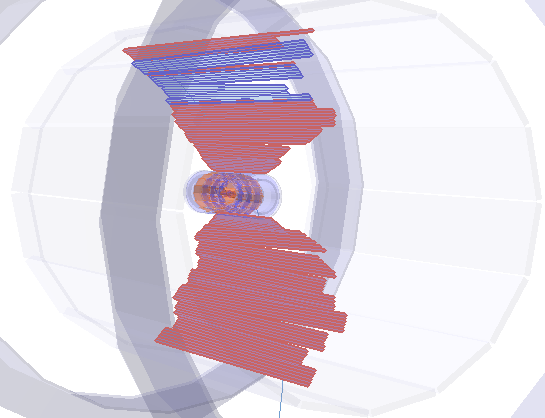
\includegraphics[width=0.6\textwidth]{figures/b2display_screenshots/gcr_data_2017-08_run3902_evt13913_finding-fail-musterevent_3d_cropped.png}
    \begin{itemize}
    \item obere Hälfte: \textcolor{kit-blue100}{Spur gefunden}
    \item untere Hälfte: \textcolor{kit-red100}{Spurfindung fehlgeschlagen}
    \end{itemize}

  \end{center}
\end{frame}

\begin{frame}
  \frametitle{Vorläufige Ergebnisse}
  % \begin{block}{}
    \begin{tabular}{ccc}
      \toprule
    Anzahl Ereignisse & gemessene Daten &  simulation Daten\\
    \midrule
    eine gefundene Spur & 1281 & 1636 \\
    zwei gefundene Spuren &  38851 & 599579\\
      \midrule
      Effizienz in Prozent& \textbf{96.8} & \textbf{99.7} \\
      \bottomrule
  \end{tabular}
% \end{block}
\begin{columns}
  \begin{column}{0.5\textwidth}
    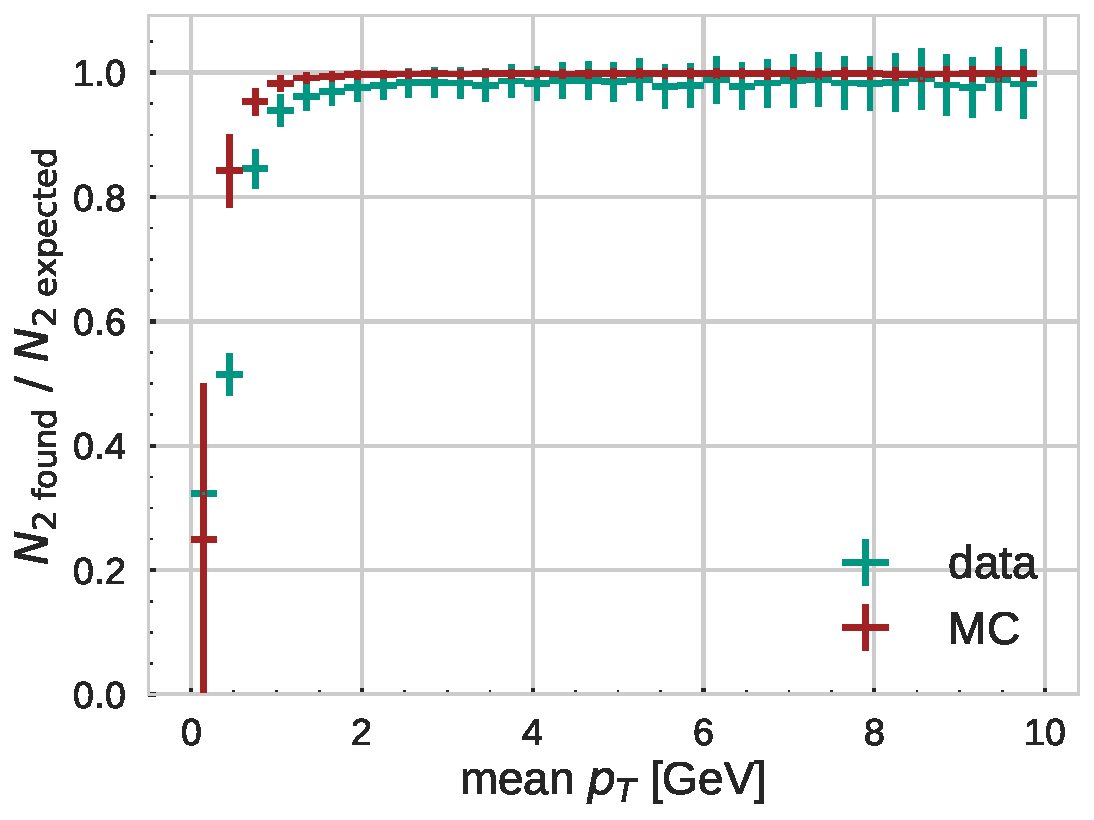
\includegraphics[width=0.8\textwidth]{figures/efficiency_study/cosmicbased_findeff_over_pt.pdf}
    \scriptsize Effizienzprofile im Transversalimpuls $p_T$
    \end{column}
  \begin{column}{0.5\textwidth}
    \begin{itemize}
    \item ähnlicher Verlauf auf gemessenen und simulierten (MC) Daten
    \item Effizienz auf gemessenen Daten etwas schlechter
    \end{itemize}
  \end{column}
\end{columns}
\end{frame}

% \begin{frame}
%   \frametitle{Effizienz-Profil in weiteren Spurparametern}
%   \begin{columns}
%     \begin{column}{0.5\textwidth}
%       \centering
%       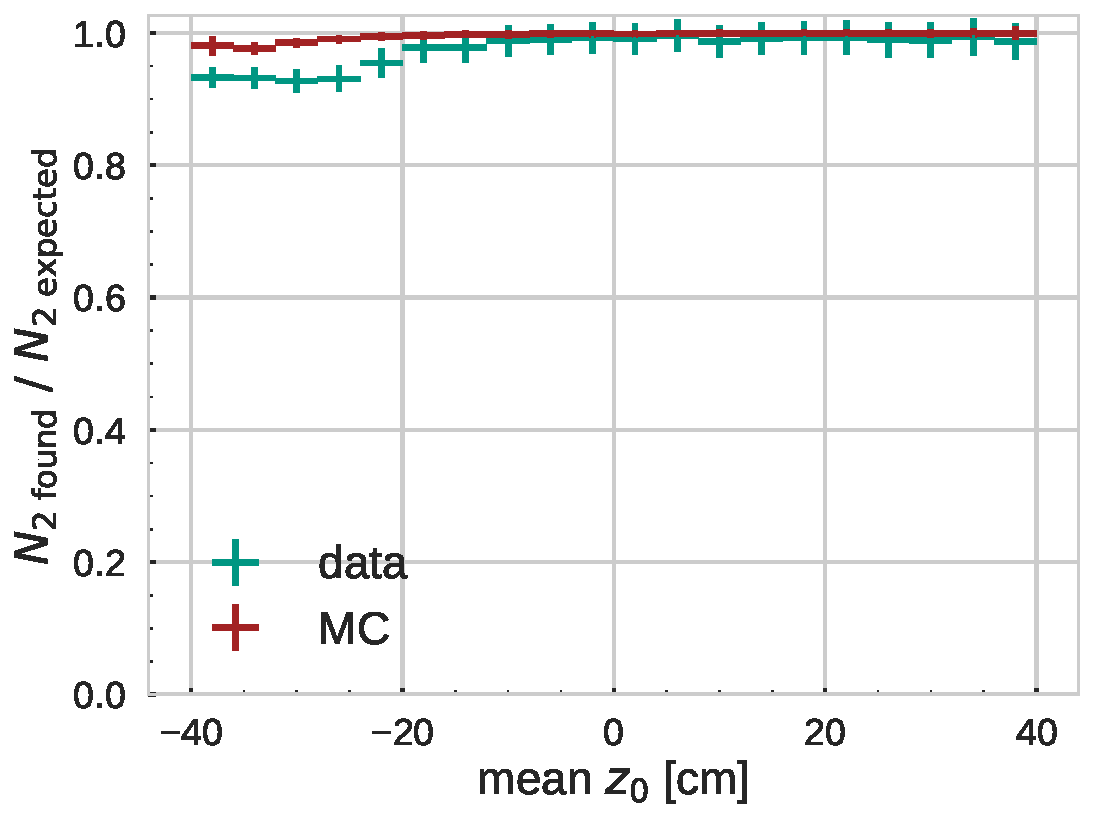
\includegraphics[width=0.85\textwidth]{figures/efficiency_study/cosmicbased_findeff_over_z0.pdf}\\
%       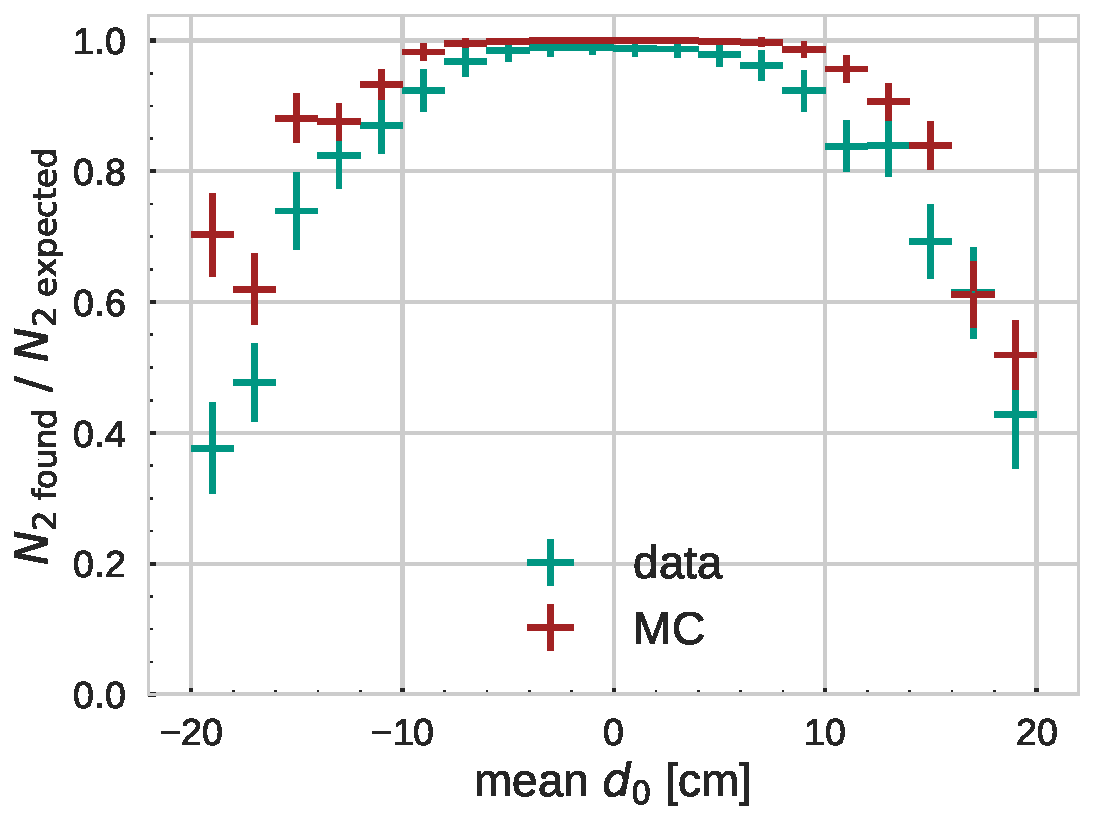
\includegraphics[width=0.85\textwidth]{figures/efficiency_study/cosmicbased_findeff_over_d0.pdf}
      
%     \end{column}
%     \begin{column}{0.5\textwidth}
%       \centering
%       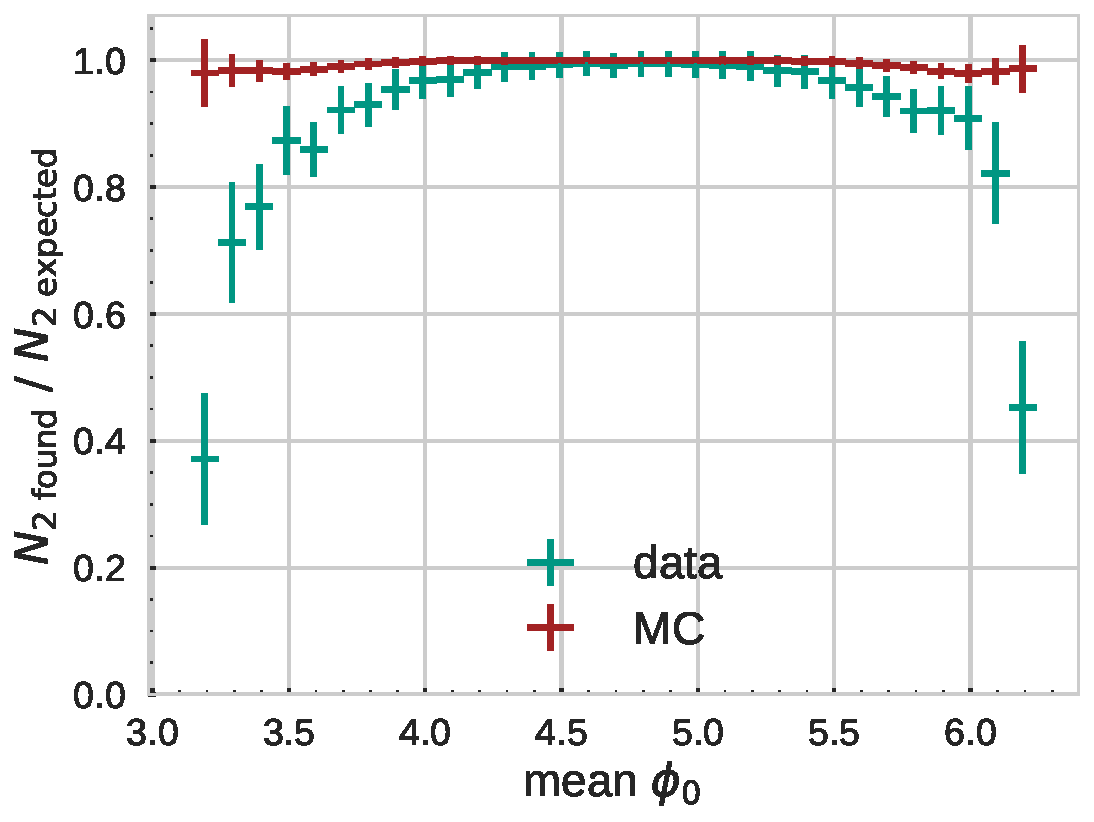
\includegraphics[width=0.85\textwidth]{figures/efficiency_study/cosmicbased_findeff_over_phi0.pdf}\\
%       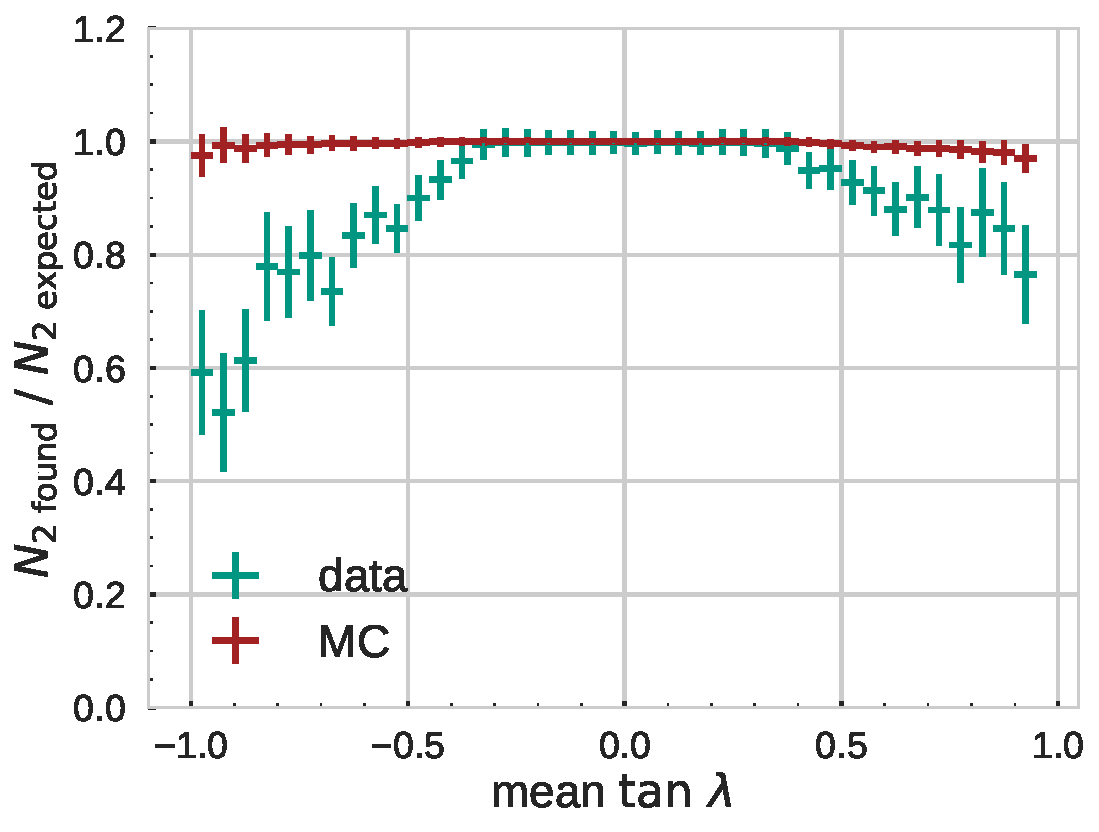
\includegraphics[width=0.85\textwidth]{figures/efficiency_study/cosmicbased_findeff_over_tan_lambda.pdf}
%     \end{column}
%   \end{columns}
% \end{frame}

\begin{frame}
  \frametitle{Fazit}
  \begin{itemize}
  \item Die Spurfindungseffizienz kann mithilfe kosmischer Myonen abgeschätzt werden.
  \item hohe Effizienz bei Impulsen über 1\,GeV, darunter erwarteter Abfall\\
  \item Schlechter auf Messdaten als auf simulierten Daten:\\
    Auswirkung einer unzureichenden Untergrundsimulation?  
  \end{itemize}
\end{frame}

\backupbegin
\begin{frame}\label{lastbeforebackup}
  \frametitle{Referenzen}
  \printbibliography
\end{frame}
\end{document}

%%% Local Variables:
%%% mode: latex
%%% TeX-master: t
%%% End:
